\documentclass[a4paper,10pt]{article}

%\usepackage[utf8]{inputenc}
\usepackage[top=2cm, bottom=2cm, left=2cm, right=2cm]{geometry}

\usepackage{graphicx} %%For loading graphic files
\usepackage{hyperref}
\graphicspath{ {Pics/} }
%\DeclareGraphicsExtensions{.png,.pdf}


\begin{document}


\title{Global Audio Manager Manual}
\author{Baranger - Holsnyder}
%\date{} %%If commented, the current date is used.
\maketitle

\clearpage


\tableofcontents %Table of contents

\clearpage



\section*{Introduction}

GAM is a set of tools designed to optimize and speed up audio integration.

\section{Arborescence}

A file hierarchy has been set up to allow for an optimized, faster audio integration in your Unity project. This hierarchy represents a conform audio structure, split into three domains : Voice, Sound Effects (SFX) and Music (see \nameref{sec:gen}).


\section{Audio Clip Manager}

The Audio Clip Manager is a file browser designed specifically to allow a global view of all audio assets and optimize their management. All audio and import settings associated with an AudioClip, along with platform-specific options, can be managed here.


\section{UI}

The UI Utility automatically references all the UI objects which are liable to play a sound on user interaction, and allows to define and control these sounds and their play settings.


\section{Music}

Easy integration of a mono or stereo dynamic music. \
The example shows the structural slicing of an 8-bit version of the Tetris music. \
More advanced options can be used to create a multitrack randomized music with the same slicing method. The example shows the process of creating such a music from a gypsy-jazz version of the same Tetris music.


\section{Switch} \label{sec:switch}

Fundamental tool of the sound designer. The Switch allows for variation on sound samples, and is frequently used on sounds which tend to be repetitive, like footsteps, or the sound of a water drop. Without this, the game can only sound artificial and poor.

\section{Animation}

Utility allowing for in-editor animation preview with sound and sound event addition and synchronization on the animation timeline. This utility allows for a classic \textit{play switch} event (see \autoref{sec:switch}), or for a \textit{play switch on surface} event, which automatically detects the surface under the animated object and plays a corresponding switch. The latter can typically be used for automatic surface-dependent footstep sounds on animated characters.


\section{Generalities} \label{sec:gen}

Audio design in a video game is made up of several layers : \begin{itemize}
\item Music.
\item Environment Sound Effects : 
	\begin{itemize}
	\item Background : non-spatialized, 2D sounds.
	\item Objects : spatialized, 3D sounds.
	\end{itemize}
\item Action SFX.
\item UI SFX.
\item Voices.
\end{itemize}


\subsection{Non-spatialized sounds}
Unity calls these 2D sounds. DO NOT mistake that for a 2D-game-exclusive instruction. Both 2D and 3D sounds should be used for any Unity project. \
A non-spatialized sound is played back directly by the sound engine, without any processing from Unity, exactly like if it were played by a regular media player. This setting is often (but not systematically) used for music, voices and background SFX. \\

\paragraph{Example} : Jardin, arbres, oiseaux, fontaine.\
Background : Birds in the trees. More or less present depending on the time of day.


\subsection{Fixed spatialized sounds}
Fixed spatialized sounds are used for objects which don't move. Nevertheless, if the listener moves, their volume will change accordingly.

\paragraph{Example} : Jardin, arbres, oiseaux, fontaine.\
Fixed spatialized sound : the fountain. It emits sound, and the player can get closer or farther. So the fountain will have an audio source, with a volume rolloff curve. For a classic, realistic rolloff, the curve should be an invert-type function : \

\begin{figure}[h]
\centering
\caption{2D object rolloff.}
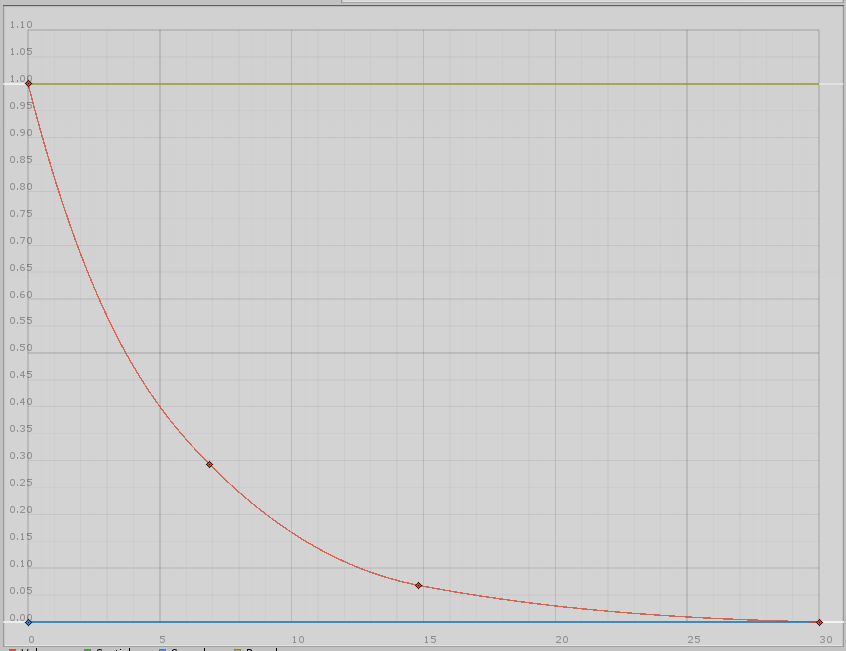
\includegraphics[width=0.5\linewidth]{logRolloff}
\end{figure}



\subsection{Mobile spatialized sounds}
A spatialized sound may be attached to a moving object.
\paragraph{Example: } Jardin, arbres, oiseaux, fontaine. A crow passes overhead and sticks around. To achieve realism, 3 elements are necessary : \begin{itemmize}
\item A switch with 2 cawing sounds at the least.
\item A Doppler effect to add to the feeling of changing distance.
\item A volume rolloff of the type :\
\end{itemize}

\begin{figure}[h]
\centering
\caption{Invert function rolloff.}
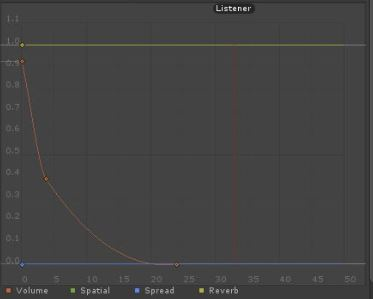
\includegraphics[width=0.4\linewidth]{dopplerRolloff}
\end{figure}




\appendix
%This is a useless appendix

\end{document}

